% Compile with XeLaTeX from docs/report. Template typography is centralized.
\documentclass[12pt,a4paper,oneside]{report}
\usepackage{fontspec}
\setmainfont{Times New Roman}
\setsansfont{Arial}
\setmonofont{Consolas}[Scale=0.85]
\usepackage[left=1.2in,right=1in,top=1.2in,bottom=1in,headheight=14pt,headsep=0.2in]{geometry}
\usepackage{amsmath,amssymb,graphicx,setspace,titlesec,caption,booktabs,array,fancyhdr,float}
\usepackage[hidelinks]{hyperref}
\onehalfspacing
\setlength{\parindent}{0pt}
\setlength{\parskip}{6pt}
\setlength{\emergencystretch}{2em}
\setlength{\abovedisplayskip}{7pt}
\setlength{\belowdisplayskip}{7pt}
\setlength{\textfloatsep}{12pt}
\setlength{\floatsep}{10pt}
\setlength{\intextsep}{12pt}
\renewcommand{\topfraction}{0.9}
\renewcommand{\bottomfraction}{0.85}
\renewcommand{\textfraction}{0.05}
\renewcommand{\floatpagefraction}{0.8}
\setcounter{bottomnumber}{3}
\renewcommand{\thechapter}{\arabic{chapter}}
\titleformat{\chapter}[display]{\centering\bfseries}{\fontsize{14}{21}\selectfont CHAPTER \Roman{chapter}}{18pt}{\fontsize{16}{24}\selectfont}
\titlespacing*{\chapter}{0pt}{0pt}{36pt}
\titleformat{\section}{\bfseries\fontsize{14}{21}\selectfont}{\thesection}{0.55em}{}
\titlespacing*{\section}{0pt}{12pt}{6pt}
\titleformat{\subsection}{\bfseries\fontsize{12}{18}\selectfont}{\thesubsection}{0.55em}{}
\titlespacing*{\subsection}{0pt}{12pt}{6pt}
\DeclareCaptionFont{template}{\fontsize{11}{16.5}\selectfont}
\captionsetup{font=template,labelfont=normalfont,justification=centering,singlelinecheck=false,skip=6pt}
\captionsetup[figure]{position=bottom}
\captionsetup[table]{position=top}
\pagestyle{fancy}\fancyhf{}\fancyfoot[C]{\thepage}
\renewcommand{\headrulewidth}{0pt}\renewcommand{\footrulewidth}{0pt}
\fancypagestyle{plain}{\fancyhf{}\fancyfoot[C]{\thepage}\renewcommand{\headrulewidth}{0pt}}
\fancypagestyle{cover}{\fancyhf{}\fancyhead[L]{\fontsize{12}{18}\selectfont Project/Thesis No.:}\renewcommand{\headrulewidth}{0pt}}
\hypersetup{pdftitle={Voyager 2 Solar-System Explorer: Computer Graphics Project Report},pdfauthor={Sarwad Hasan Siddiqui}}
\graphicspath{{figures/}{figures/technical/}}
\newcommand{\code}[1]{\texttt{#1}}
\newcommand{\frontheading}[1]{\begin{center}\bfseries\fontsize{16}{24}\selectfont #1\end{center}\vspace{18pt}}
\newcommand{\plate}[2]{\begin{figure}[H]\centering\includegraphics[width=\textwidth]{#1}\caption{#2}\label{fig:\thefigure}\end{figure}}
\newcommand{\para}[1]{\par\vspace{12pt}\noindent#1\par}
\newcommand{\manualpage}{\clearpage}
\begin{document}

% The original cover specifies its own top and header positions.
\newgeometry{left=1.2in,right=1in,top=1.2in,bottom=1in,headheight=18pt,headsep=32pt}
\thispagestyle{cover}
\begin{center}
{\fontsize{14}{21}\selectfont CSE 4102: Computer Graphics and\\Image Processing Laboratory\par}
\vspace{18pt}
{\fontsize{18}{27}\selectfont\bfseries\scshape Voyager 2 Solar-System Explorer\\An Interactive Three-Dimensional\\Computer Graphics Project\par}
\vspace{36pt}
{\fontsize{14}{21}\selectfont By\par}
\vspace{54pt}
{\fontsize{14}{21}\selectfont\bfseries Sarwad Hasan Siddiqui\par}
{\fontsize{14}{21}\selectfont Roll: 2107006\par}
\vspace{36pt}

\includegraphics[width=1.14in,height=1in,keepaspectratio]{KUET-LOGO.png}
\vfill
{\fontsize{12}{14.4}\selectfont\bfseries Department of Computer Science and Engineering\\
Khulna University of Engineering \& Technology\\
Khulna 9203, Bangladesh\\October, 2026\par}
\end{center}
\manualpage\restoregeometry\normalsize\pagenumbering{roman}

\begin{center}
{\fontsize{18}{27}\selectfont\bfseries Voyager 2 Solar-System Explorer\\An Interactive Three-Dimensional\\Computer Graphics Project\par}
\vspace{54pt}
By\par\vspace{36pt}
\textbf{Sarwad Hasan Siddiqui}\\Roll: 2107006\par
\vspace{30pt}
A project report submitted for\\
\textbf{CSE 4102}\\
Computer Graphics and Image Processing Laboratory\par
\end{center}
\vspace{24pt}
\textbf{Course Teachers:}\par
\hspace*{0.8in}\begin{minipage}{0.8\textwidth}
\textbf{Md Tajmilur Rahman}\\Lecturer\\
Department of Computer Science and Engineering\\
Khulna University of Engineering \& Technology\par\vspace{12pt}
\textbf{Md Mubtashim Abrar Nihal}\\Lecturer\\
Department of Computer Science and Engineering\\
Khulna University of Engineering \& Technology
\end{minipage}
\vfill
\begin{center}Department of Computer Science and Engineering\\Khulna University of Engineering \& Technology\\Khulna 9203, Bangladesh\\October, 2026\end{center}
\manualpage

\frontheading{Acknowledgment}
\para{I thank the course teachers, Md Tajmilur Rahman and Md Mubtashim Abrar Nihal, for the opportunity to develop and present this Computer Graphics and Image Processing Laboratory project. Preparing the explorer required connecting mathematical models to visible, controllable results: a mesh must have valid triangles, a transform must preserve its hierarchy, and a lighting equation must produce an explainable image.}
\para{NASA and JPL provide the mission information, spacecraft reference material and Horizons state vectors used by the project. Solar System Scope provides the credited body maps. GLFW, GLAD and GLM support the Windows/OpenGL implementation. Their documentation and original graphics publications are identified in the references.}
\para{This report distinguishes sourced assets and standard algorithms from the project's own procedural geometry, scene organization, data integration and rendering choices. Runtime screenshots demonstrate implemented behavior; construction diagrams explain the corresponding mathematics.}
\vspace{18pt}\begin{flushright}\textbf{Sarwad Hasan Siddiqui}\end{flushright}
\manualpage

\frontheading{Abstract}
\para{Voyager 2 Solar-System Explorer is an interactive C++20 and OpenGL application that combines an educational solar-system scene with historical spacecraft playback and manual flight. Its purpose is to make computer-graphics fundamentals visible through objects that can be inspected, moved and rendered under controlled comparisons. The scene contains 26 textured celestial bodies, four planetary ring systems, a procedurally constructed Voyager 2, 8,500 instanced small bodies, a comet, orbit guides, a starfield, mission-path lines and heliosphere boundaries.}
\para{The geometry is generated from reusable indexed primitives rather than an imported spacecraft model. A shared latitude--longitude sphere provides body vertices, normals and texture coordinates. Boxes, cylinders, frustums, rods and a closed parabolic dish form 76 spacecraft assemblies containing 5,828 triangles. Scene-graph transforms preserve assembly and moon relationships; double-precision world positions and a floating origin support both spacecraft close-ups and large-scale navigation.}
\para{Offline NASA/JPL Horizons position and velocity samples drive planets and Voyager on one date through cubic Hermite interpolation. Moon revolution and axial spin use separate visual rates. The user can switch among four camera modes, inspect 18 spacecraft components, control time, select objects and pilot the probe with quaternion-based six-degree-of-freedom motion.}
\para{The lighting system implements a Sun point light, camera-attached spotlight and directional fill. Five raster shading techniques share the light model. Albedo maps, derived normal maps, an ocean specular mask and a NASA spacecraft atlas provide surface detail. Analytic sphere/ring shadow rays, a spacecraft shadow map and a hybrid Whitted view demonstrate visibility and reflection. A surface-area-heuristic triangle BVH accelerates the traced spacecraft.}
\para{Debug and Release builds, repository checks, runtime captures and input regression evidence accompany the submission. Eight uncapped Release views measured 0.64--6.60 ms per frame on the observed Radeon RX 590 at 1440 by 900. These measurements describe one machine and run. The report states the educational scale compression, visual moon phases and limited ray-tracing scope explicitly.}
\manualpage

\frontheading{Contents}
\begin{spacing}{1.2}
\begin{tabular}{@{}p{0.85\textwidth}r@{}}
Title Page & i\\Acknowledgment & ii\\Abstract & iii\\Contents; Lists of Tables and Figures & iv\\[6pt]
CHAPTER I\quad Introduction & \pageref{ch:intro}\\
CHAPTER II\quad Background and System Design & \pageref{ch:background}\\
CHAPTER III\quad Methodology & \pageref{ch:method}\\
\quad Indexed geometry and curved surfaces & \pageref{sec:geometry}\\
\quad Spacecraft and environment construction & \pageref{sec:objects}\\
\quad Transforms, cameras and presentation scale & \pageref{sec:transforms}\\
\quad Historical, orbital and manual motion & \pageref{sec:motion}\\
\quad Lighting; shading; textures & \pageref{sec:lighting}--\pageref{sec:textures}\\
\quad Shadow rays, Whitted tracing and triangle BVH & \pageref{sec:rays}\\
CHAPTER IV\quad Implementation, Results and Discussion & \pageref{ch:results}\\
CHAPTER V\quad Societal and Professional Considerations & \pageref{ch:impacts}\\
CHAPTER VI\quad Complex Engineering Problems and Activities & \pageref{ch:engineering}\\
CHAPTER VII\quad Conclusions & \pageref{ch:conclusion}\\References & \pageref{references}
\end{tabular}
\end{spacing}
\vspace{12pt}{\centering\bfseries\fontsize{16}{24}\selectfont List of Tables\par}
\begin{spacing}{1.2}
3.1 Geometry counts (p.\,\pageref{tab:mesh}); 4.1 benchmark (p.\,\pageref{tab:benchmark}).
\end{spacing}
\vspace{12pt}{\centering\bfseries\fontsize{16}{24}\selectfont List of Figures\par}
\begin{spacing}{1.2}
1.1 Overview (p.\,\pageref{fig:1.1}); 2.1 pipeline (p.\,\pageref{fig:2.1}); 3.1 indexed cell (p.\,\pageref{fig:3.1}); 3.2 primitive construction (p.\,\pageref{fig:3.2}); 3.3 hierarchy (p.\,\pageref{fig:3.3}); 3.4 motion (p.\,\pageref{fig:3.4}); 3.5 lights (p.\,\pageref{fig:3.5}); 3.6 shading (p.\,\pageref{fig:3.6}); 3.7 maps (p.\,\pageref{fig:3.7}); 3.8 rays (p.\,\pageref{fig:3.8}).
\end{spacing}
\manualpage\pagenumbering{arabic}

\chapter{Introduction}\label{ch:intro}
\section{Purpose and scope}
\para{The explorer connects graphics fundamentals to inspectable results: procedural objects, hierarchical transforms, historical flybys, manual flight and raster/traced comparisons. Floating-origin precision and educational scale mappings make metre-scale hardware visible beside planets and multi-AU trajectories.}
\para{Its scene contains 26 bodies, four ring systems, 76 spacecraft assemblies with 18 inspection targets, 8,500 rocks, a comet, 7,380 stars, orbit/path guides and heliosphere boundaries. Work proceeds through geometry, hierarchy, mission/navigation, spacecraft, lighting/tracing and verification. The contribution is this integration; standard algorithms are credited, not claimed as new research.}
\plate{report_overview.png}{Runtime overview: labelled bodies and orbit guides organize exploration. Telemetry bands are cropped for print.}
\manualpage

\chapter{Background and System Design}\label{ch:background}
\section{From geometry to pixels}
\para{Indexed vertices hold position, normal and UV. The vertex shader transforms them; rasterization covers pixels and interpolates attributes; the fragment shader evaluates material and lighting. Depth testing preserves nearer surfaces. Transparent rings/glow blend after opaque objects without depth writes. Lines and points use separate primitive modes \cite{opengl}.}
\section{Architecture and data ownership}
\para{The loop is input $\rightarrow$ update $\rightarrow$ render. \code{Window} owns GLFW; \code{Input} polls events. Scene nodes own children; shared RAII meshes/textures avoid duplicate uploads. \code{MissionController} owns dated placement; camera/light controllers change viewing state. CSV catalogues separate physical data from geometry. Shaders share \code{lighting.glsl}.}
\para{Instancing reduces draws. Double-precision floating origin and log depth stabilize close-ups; one date keeps flybys coherent. A triangle BVH handles hardware while cheap guides remain rasterized.}
\begin{figure}[H]\centering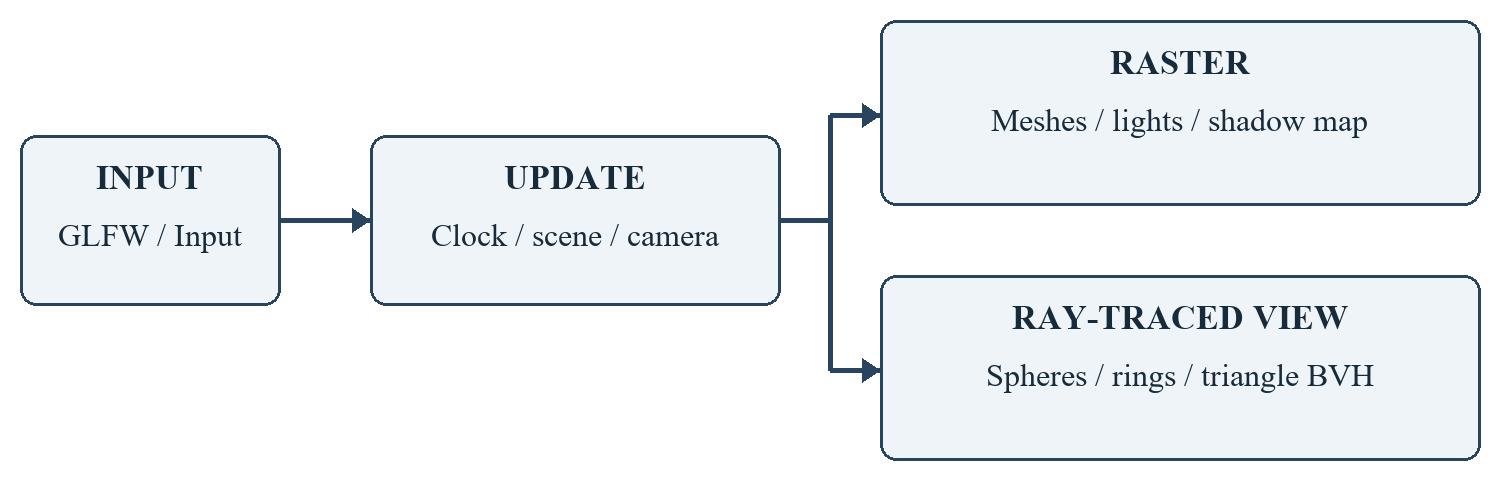
\includegraphics[width=\textwidth]{architecture.png}\caption{Controllers update a shared scene; raster and traced paths consume its state.}\label{fig:2.1}\end{figure}
\manualpage

\chapter{Methodology}\label{ch:method}
\section{Indexed geometry and curved surfaces}\label{sec:geometry}
\para{Each 32-byte vertex stores position, normal and UV at locations 0, 1 and 2. A VBO holds records, an EBO unsigned indices and a VAO their interpretation. For sphere latitude $i/L$ and longitude $j/N$, define $\phi=\pi i/L$ and $\theta=2\pi j/N$:}
\begin{equation}
\mathbf p=(\sin\phi\cos\theta,\cos\phi,\sin\phi\sin\theta),\quad
\mathbf n=\mathbf p,\quad (u,v)=(1-j/N,1-i/L).
\end{equation}
\para{Each interior cell emits $(TL,TR,BL)$ and $(TR,BR,BL)$, where $TL=i(N+1)+j$, $TR=TL+1$, $BL=TL+N+1$ and $BR=BL+1$. The north/south zero-area halves are omitted. With $L=32,N=64$, $(L+1)(N+1)=2,145$ vertices produce $2N(L-1)=3,968$ triangles and 11,904 indices. Seam positions repeat with distinct $u=0,1$; otherwise texture interpolation would cross the map incorrectly.}
\plate{index_cell.png}{One indexed sphere cell: two triangles share records and an edge. Winding is counter-clockwise from outside.}


\section{Spacecraft and environment construction}\label{sec:objects}
\para{A box has 24 face-specific vertices and 12 triangles: $(b,b+1,b+2)$, $(b,b+2,b+3)$ per face. Cylinder/frustum rings use $(r_k\cos\theta,\pm h/2,r_k\sin\theta)$; side normals are proportional to $(h\cos\theta,r_b-r_t,h\sin\theta)$. Separate cap fans preserve hard normals. Both capped nonzero radii give $4n+6$ vertices and $4n$ triangles.}
\para{Voyager is authored from boxes, a decagonal cylindrical bus, rods, frustums and a parabolic dish. Its metre dimensions share the factor 0.006 render units/metre. For dish radius $R$, depth $D$ and radial coordinate $r$, the front profile and normal follow the surface derivative:}
\begin{equation}
y=-D+D(r/R)^2,\qquad
\mathbf n=\operatorname{normalize}(-2Dr\cos\theta/R^2,1,-2Dr\sin\theta/R^2).
\end{equation}
\para{The rear surface is offset by thickness and has reversed normals/winding. Center fans, radial quads and a joined rim form a closed shell. The current $48\times6$ dish has 590 vertices and 1,152 triangles. Merged parts transform positions and inverse-transpose normals, then add the destination vertex offset to every appended index. A rod uses midpoint $(A+B)/2$, height $|B-A|$ and rotation from $+Y$ to $B-A$.}
\begin{table}[H]\caption{Other primitive counts and their scene uses.}\label{tab:mesh}\centering
\begin{spacing}{1.0}\begin{tabular}{@{}p{0.37\textwidth}p{0.58\textwidth}@{}}\toprule
Primitive & Counts / use\\\midrule
Double-sided annulus & 260 vertices, 256 triangles per 64-segment band\\
Low-poly sphere & 28 vertices, 24 triangles per instanced rock\\
Star points / circle & 7,380 points / 96 line vertices; zero triangles\\
Comet cone & 52 vertices, 32 triangles; sphere nucleus and coma\\\bottomrule
\end{tabular}\end{spacing}\end{table}
\para{Rings use $(r\cos\theta,0,r\sin\theta)$, separate top/bottom normals and inner/outer edges. Uniform $\cos\phi$ avoids star polar clustering. Static rocks vary their matrices; the comet tail points anti-Sun. Orbit/path lines, six heliosphere great circles and glyph quads complete the families.}
\plate{primitive_profiles.png}{Authored construction diagrams: face-separated box, capped cylinder and the current six-ring parabolic dish.}


\section{Transforms, cameras and presentation scale}\label{sec:transforms}
\para{Column-vector transforms act right to left: scale in object space, rotate, then translate. Children inherit the parent matrix, so one spacecraft root moves all assemblies together:}
\begin{equation}
M_{local}=TRS,\quad M_{world}=M_{parent}M_{local},\quad
\mathbf n' = \operatorname{normalize}((M_{3\times3}^{-1})^T\mathbf n).
\end{equation}
\para{Normals use the inverse-transpose because nonuniform scale changes the perpendicular direction. Planets store orbit position and axial tilt in the parent frame. Their sphere alone receives spin; moons and rings inherit the unspun frame. Moon local position and scale are divided by parent radius to compensate for inherited scaling.}
\begin{equation}\begin{aligned}
R_{body}&=0.50(R_{km}/6371)^{0.60},\quad R_{Sun}\leq6,\\
d_{render}&=12(d_{AU}/0.387098)^{0.55},\\
d_{moon}&=R_{parent}\left(1.6+\sqrt{a_{km}/R_{parent,km}}\right).
\end{aligned}\end{equation}
\para{These monotonic laws preserve ordering while increasing visibility. They are display mappings, not physical scale. Before narrowing to float, the renderer subtracts the eye in double precision. Projection uses a camera-relative view and logarithmic depth $z=\log_2(1+w)/\log_2(1+far)$.}
\para{FreeFly moves independently; Focus orbits a body; Chase orbits in Voyager's frame; Inspect targets the craft or one of 18 components. Orbit cameras convert yaw, pitch and radius into an offset, rotate it by their frame and aim at the target. Smooth transitions avoid jumps. Picking builds a screen ray and compares angular body/spacecraft bounds.}
\plate{transform_hierarchy.png}{Surface spin does not rotate the planet's children. The floating origin is applied consistently to geometry, lights and ray primitives.}


\section{Historical, orbital and manual motion}\label{sec:motion}
\para{Horizons rows provide Julian date, heliocentric position and velocity in AU/day \cite{horizons}. With normalized interval time $s=(JD-JD_0)/h$, cubic Hermite interpolation matches both endpoints and velocities:}
\begin{equation}\begin{aligned}
\mathbf p(s)={}&(2s^3-3s^2+1)\mathbf p_0+(s^3-2s^2+s)h\mathbf v_0\\
&+(-2s^3+3s^2)\mathbf p_1+(s^3-s^2)h\mathbf v_1.
\end{aligned}\end{equation}
\para{One date drives planets and Voyager. Ecliptic $(x,y,z)$ maps to $(x,z,y)$ before compression. Smooth flyby clearance prevents intersection with enlarged planets. After 2030, planets use $E-e\sin E=M$ two-body continuation; Voyager is ballistic. These are approximate predictions.}
\begin{equation}
r=\frac{a(1-e^2)}{1+e\cos\nu},\quad
\nu\gets\nu+\frac{2\pi(0.4)}{P_{days}}\Delta t\,speed,\quad
\psi\gets\psi+\frac{2\pi}{P_{hours}}\Delta t\,speed.
\end{equation}
\para{Moon phases and spin are visual rates; their signed periods produce retrograde cases. Moons use constant true-anomaly speed, unlike the dated planets. The comet uses an ellipse and rotates its tail from $+Y$ toward $\operatorname{normalize}(p_{comet}-p_{Sun})$. Manual flight uses real time, inertial translation and body-axis quaternion rotation:}
\begin{equation}
q\gets\operatorname{normalize}(q\,q_yq_xq_z),\quad
\mathbf v\gets\mathbf v+\mathbf a\Delta t,\quad \mathbf p\gets\mathbf p+\mathbf v\Delta t.
\end{equation}
\para{Velocity need not face forward. Braking cannot reverse it; speed is capped at 12 units/s. $P$ pauses astronomical motion while cameras and manual flight remain usable.}
\plate{moon_motion.png}{Runtime Jupiter sequence: moons move independently in the tilted planetary frame; body spin does not drag their orbits.}


\section{Lighting: three types and a moving light}\label{sec:lighting}
\para{At surface point $p$, $n$ is the unit normal and $v$ points to the eye. A point light uses $l=(p_L-p)/|p_L-p|$; a directional light uses the same $l=-d_L$ everywhere. The Sun is a point light. The cool fill is directional and has no distance falloff. The spotlight is at the camera and follows its forward direction. Its motion therefore changes illumination when the eye moves.}
\begin{equation}
A(d)=\frac{1}{\max(k_c+k_ld+k_qd^2,10^{-4})},\qquad D=\max(n\cdot l,0).
\end{equation}
\para{The optional Sun attenuation is $1/[0.3+0.7(d/20)^2]$, equal to one at $d=20$. Default constant intensity keeps outer bodies readable. For the camera headlamp, intensity is 1.4, quadratic reach is three times nearest-surface distance, and the soft cone spans $12^\circ$--$18^\circ$:}
\begin{equation}
C=\operatorname{clamp}\left(\frac{(-l)\cdot d_L-\cos18^\circ}{\cos12^\circ-\cos18^\circ},0,1\right),\quad I_L=colour\cdot intensity\cdot A\cdot C.
\end{equation}
\para{Only spotlights use $C$; it is one for other types. With ambient 0.07, albedo $a$ and Sun visibility $V_S$, the renderer keeps the Sun and other terms separate:}
\begin{equation}
I=a(0.07+V_SD_S+D_{other})+V_SS_S+S_{other}.
\end{equation}
\para{Thus an eclipse removes Sun illumination while the headlamp and fill still work. Two-sided rings use $|n\cdot l|$. $K$ toggles lighting; $F5,F6,F7$ toggle headlamp, fill and Sun falloff. Inspect provides a camera-related studio fill to reveal hardware. Neither auxiliary light casts shadows.}
\plate{report_lighting.png}{Same frozen Moon and camera: Sun only, added spotlight, added directional fill. The Sun stays enabled in all three comparisons.}


\section{Shading: where and how light is evaluated}\label{sec:shading}
\para{Lighting defines the source geometry; shading defines the surface normal and evaluation stage. The five $F3$ modes share diffuse $D=\max(n\cdot l,0)$, material specular strength $k_s$ and power $p$. Phong uses the reflected light direction; Blinn--Phong uses the halfway direction:}
\begin{equation}
r=2(n\cdot l)n-l,\quad S_P=k_s\max(v\cdot r,0)^p,
\quad h=\frac{l+v}{|l+v|},\quad S_B=k_s\max(n\cdot h,0)^{2p}.
\end{equation}
\para{Flat derives one face normal from $\operatorname{normalize}(\partial_xp\times\partial_yp)$, revealing facets. Gouraud evaluates Phong lighting at vertices and interpolates terms across the triangle; highlights between vertices can be lost. Phong evaluates per pixel with an interpolated, normalized normal. Blinn--Phong uses the half-vector per pixel; doubling the exponent is this implementation's approximate highlight-size match.}
\begin{equation}
D_{toon}=\begin{cases}1& D>0.75\\0.62&D>0.40\\0.30&D>0.12\\0.06&\text{otherwise}\end{cases}
\end{equation}
\para{Toon quantizes positive diffuse light into these bands, thresholds specular at 0.5 and draws rim ink when $n\cdot v<0.22$. The unlit back side remains zero diffuse. Gouraud disables normal maps because the derived detail belongs to fragments. Unlit objects use colour/texture without illumination. Glow uses $\alpha=|n\cdot v|^p\,opacity$ and additive blending for Sun and comet shells; it is a material behavior, not a sixth selectable shading technique.}
\plate{report_shading.png}{Earth in the same frozen view under Flat, Gouraud, Phong, Blinn--Phong and Toon. The presentation also shows matching spacecraft comparisons.}


\section{Textures and derived surface detail}\label{sec:textures}
\para{Albedo and transforms distinguish 26 bodies. UVs duplicate the seam and preserve north/south orientation. Loading flips image rows; filtering/mipmaps reduce minification artifacts. NASA and Solar System Scope are credited \cite{textures,nasaassets}.}
\para{Voyager uses NASA hardware imagery in an atlas, not imported NASA geometry. A material selects a rectangle through $uv'=uv\cdot zw+xy$. Eleven textured finishes share the atlas; copper is untextured. Thus foil wrinkles and louvres change surface appearance while the procedural mesh supplies the silhouette.}
\begin{equation}
H=0.2126R+0.7152G+0.0722B,\quad
n_t=\operatorname{normalize}(-s\,S_x(H),-s\,S_y(H),1).
\end{equation}
\para{The Sobel horizontal kernel has rows $(-1,0,1)$, $(-2,0,2)$, $(-1,0,1)$; the vertical kernel is its transpose. Longitude wraps and latitude clamps. Encode $(n_t+1)/2$. Screen derivatives of position/UV reconstruct the tangent frame, transforming sampled normals into the lighting frame without a tangent attribute. This colour-derived relief does not measure elevation or move vertices.}
\para{Earth's mask marks water if $B>1.25R$, $B>1.02G$, $R+G+B<1.5$, assigning 255 versus 30. $F8$ toggles maps. Tracing uses 26 $1024\times512$ albedo layers and omits raster normal/specular maps.}
\begin{figure}[H]\centering
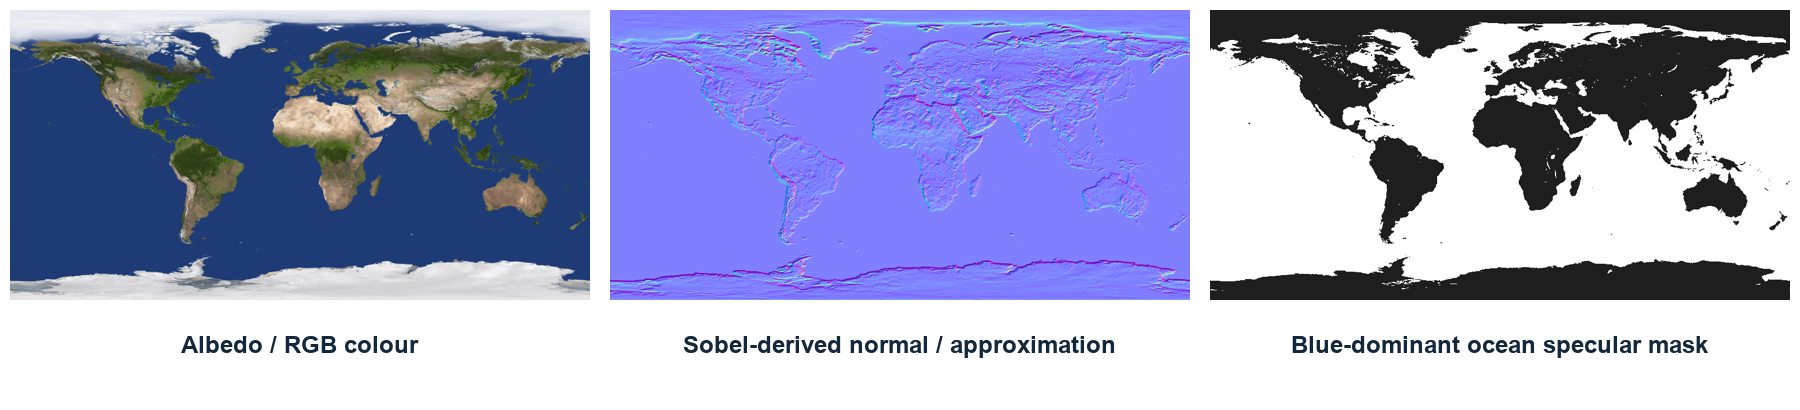
\includegraphics[width=\textwidth]{texture_channels.png}\par\vspace{6pt}
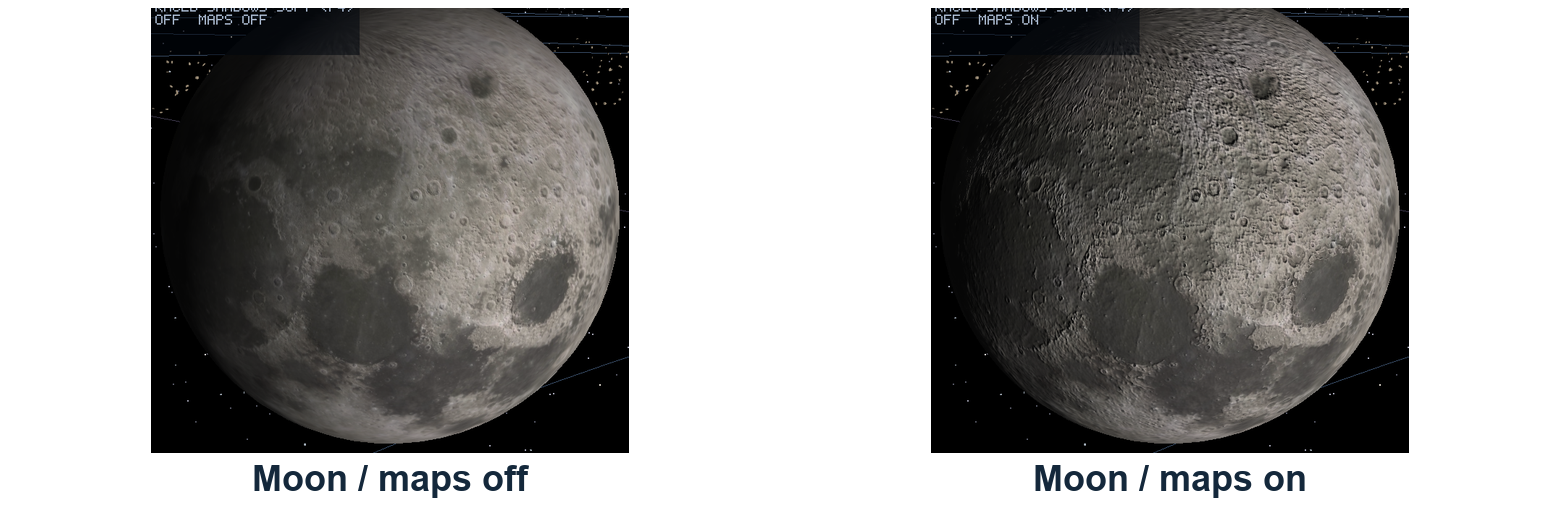
\includegraphics[width=\textwidth]{report_surface_maps.png}
\caption{Derived Earth channels (top); runtime Moon maps off/on (bottom). Normal maps change illumination, not the silhouette.}\label{fig:3.7}\end{figure}


\section{Shadow rays, Whitted tracing and triangle BVH}\label{sec:rays}
\para{For $p(t)=o+td$ with unit $d$, a sphere satisfies $|p-c|^2=R^2$. Define $b=(o-c)\cdot d$ and $f=|o-c|^2-R^2$; its roots are $t=-b\pm\sqrt{b^2-f}$. Reject a negative discriminant and choose the nearest positive root. A ring intersects its plane:}
\begin{equation}
t=\frac{(c-o)\cdot N}{d\cdot N};\qquad R_{in}\leq|o+td-c|\leq R_{out}.
\end{equation}
\para{Raster Sun rays test spheres and annuli. Hard mode tests the Sun center; soft uses finite-Sun disc overlap for analytic penumbrae. Rings multiply visibility by $1-opacity$. Voyager's raster self-shadows use a $2048^2$ Sun depth map and $3\times3$ PCF depth comparisons, avoiding per-pixel BVH traversal.}
\para{$F9$ finds the nearest primitive. For triangle edges $e_1=B-A,e_2=C-A$, Möller--Trumbore defines $P=d\times e_2$, $det=e_1\cdot P$, $Q=(o-A)\times e_1$ \cite{moller}:}
\begin{equation}
u=\frac{(o-A)\cdot P}{det},\quad v=\frac{d\cdot Q}{det},\quad t=\frac{e_2\cdot Q}{det}.
\end{equation}
\para{Accept $t>0$, $u,v\geq0$, $u+v\leq1$. Weights $(1-u-v,u,v)$ interpolate UV/normal. Voyager's 12-bin SAH BVH has 5,828 triangles, 6,723 nodes and depth 24. Local-space rays traverse a 32-entry stack near-first; bounding-box slab intervals reject empty regions.}
\para{Whitted lighting uses Blinn--Phong, Sun rays, four ring layers and one optional reflection $d_r=d-2(d\cdot n)n$ \cite{whitted}, weighted by reflectivity. Reflections omit Voyager. The environment stays rasterized with shared log depth. Bias prevents self-hits; refraction and diffuse global illumination are absent.}
\plate{ray_paths.png}{Primary, shadow and reflection rays have different jobs. Tracing is hybrid, with analytic bodies and a triangle-BVH spacecraft.}


\chapter{Implementation, Results and Discussion}\label{ch:results}
\section{Verification and performance}
\para{Debug/Release builds, both repository checks, input-tap regression and runtime tours passed. Assessment captures show wireframes, lights and motion. GLFW sticky inputs latch previously missed brief taps \cite{glfw}; existing dependency linker warnings remain in the logs.}
\begin{table}[b]\caption{Release timings: RX 590, 1440 by 900, vsync off.}\label{tab:benchmark}\centering
\begin{spacing}{1.0}\begin{tabular}{@{}lrr@{}}\toprule
View & Frame ms & GPU ms\\\midrule
Overview & 0.64 & 0.42\\Launch chase & 0.83 & 0.65\\Jupiter focus & 0.68 & 0.51\\Saturn focus & 0.72 & 0.55\\Voyager inspect & 0.99 & 0.58\\Dish close-up & 1.15 & 0.96\\Saturn traced & 2.10 & 1.77\\Voyager traced & 6.60 & 5.89\\\bottomrule
\end{tabular}\end{spacing}\end{table}
\para{The eight-view mean is 1.71 ms. Sphere LOD selects 3,968/960/224 triangles by apparent size; frustum culling rejects invisible bodies. Instancing draws 8,500 rocks in three calls using 24 triangles each. Texture detail reduces spacecraft geometry. This is one measured run, not a hardware-independent guarantee. GPU query retrieval can wait; counters omit shadow-depth, tracing and HUD draws, although GPU timing includes HUD rendering.}
\section{Interaction and demonstration}
\para{$1$--$6$ select bookmarks; $P$ pauses; $=$/$-$ alter rate. $H,C,I$, Tab and brackets select camera targets. $V$ enables manual flight; $F3$--$F10$ compare rendering. The deck contains two introductions, ten technical slides and thanks. The author will attach the final video after the introduction.}
\manualpage

\chapter{Societal and Professional Considerations}\label{ch:impacts}
\para{NASA/JPL assets, credited texture licences and standard algorithms remain attributed. Scale compression, visual moon/spin rates and colour-derived relief are disclosed. The explorer is educational, not a navigation instrument. Offline assets avoid collecting user data; pause/rate controls support explanation.}
\vspace{6pt}
\refstepcounter{chapter}\label{ch:engineering}
\begin{center}{\bfseries\fontsize{14}{21}\selectfont CHAPTER VI}\par\vspace{12pt}{\bfseries\fontsize{16}{24}\selectfont Complex Engineering Problems and Activities}\end{center}\vspace{6pt}
\para{Precision, topology, hierarchy, dated motion and shader visibility interact. Shared geometry, clearance mappings, one mission date, BVH traversal and selective shadows address these constraints. Construction, integration, profiling and verification are evidenced by source, captures and timings.}
\vspace{6pt}
\refstepcounter{chapter}\label{ch:conclusion}
\begin{center}{\bfseries\fontsize{14}{21}\selectfont CHAPTER VII}\par\vspace{12pt}{\bfseries\fontsize{16}{24}\selectfont Conclusions}\end{center}\vspace{6pt}
\para{The project unites procedural geometry, mission exploration, five shaders, three lights, textures and hybrid tracing. Limits include static belts, illustrative comet motion, approximate hardware, colour-derived relief and Sun-only shadows. Tracing omits Voyager reflections, raster normal/specular maps, refraction and global illumination; post-2030 motion is approximate and the clock finite.}
\para{Future work can add measured relief, dated moons, articulation and wider shadows after profiling. Defense preparation should cover indices, normals, TRS, Hermite interpolation, quaternions, light falloff, shading stages and intersections. Manual input and target-machine rehearsal remain necessary.}
\manualpage

\renewcommand{\bibname}{REFERENCES}
\titleformat{\chapter}[block]{\centering\bfseries\fontsize{14}{21}\selectfont}{}{0pt}{}
\titlespacing*{\chapter}{0pt}{0pt}{36pt}
\begin{spacing}{1.2}
\begin{thebibliography}{9}
\label{references}
\setlength{\itemsep}{6pt}\setlength{\parskip}{0pt}
\bibitem{opengl} Khronos Group, ``The OpenGL Graphics System: A Specification,'' ver. 3.3, Mar. 2010. [Online]. Available: \url{https://registry.khronos.org/OpenGL/specs/gl/glspec33.core.pdf}
\bibitem{horizons} Jet Propulsion Laboratory, ``Horizons System Manual.'' [Online]. Available: \url{https://ssd.jpl.nasa.gov/horizons/manual.html}. Accessed: Oct. 5, 2026.
\bibitem{glfw} GLFW, ``Input Guide.'' [Online]. Available: \url{https://www.glfw.org/docs/latest/input_guide.html}. Accessed: Oct. 5, 2026.
\bibitem{textures} Solar System Scope, ``Solar System Textures,'' CC BY 4.0. [Online]. Available: \url{https://www.solarsystemscope.com/textures/}. Accessed: Oct. 5, 2026.
\bibitem{nasaassets} NASA, ``NASA 3D Resources'' and ``Voyager 2.'' [Online]. Available: \url{https://github.com/nasa/NASA-3D-Resources}; \url{https://science.nasa.gov/mission/voyager/voyager-2/}. Accessed: Oct. 5, 2026.
\bibitem{moller} T. Möller and B. Trumbore, ``Fast, minimum storage ray-triangle intersection,'' \emph{Journal of Graphics Tools}, vol. 2, no. 1, pp. 21--28, 1997, doi: 10.1080/10867651.1997.10487468.
\bibitem{whitted} T. Whitted, ``An improved illumination model for shaded display,'' \emph{Communications of the ACM}, vol. 23, no. 6, pp. 343--349, Jun. 1980, doi: 10.1145/358876.358882.
\bibitem{project} S. H. Siddiqui, ``Voyager 2 Solar-System Explorer,'' project source, object handbook, implementation bible, learning guide and validation records, KUET, Oct. 2026. Local paths: \code{src/}, \code{shaders/}, \code{docs/objects/}, \code{docs/guide/}, \code{docs/report/validation/}.
\end{thebibliography}
\end{spacing}
\end{document}
